% -----------------------------
% PERSONNALISATION DE DOCUMENTS
% -----------------------------

% Defining TOC's sections before content
\section{Personnalisation de documents}

\subsection{Mise en page}

\subsection{En-têtes, pieds de page et sections}

\begin{frame}
    \vfill
    \begin{center}
        \large
        Personnalisation de documents
    \end{center}
    \vfill
\end{frame}

\begin{frame}
    \frametitle{Personnalisation de documents - Mise en page}
    Module \textcolor{vibrant_green}{\textit{geometry}}\footnotemark permet de gérer les dimensions des pages.
    \begin{figure}
        \centering
            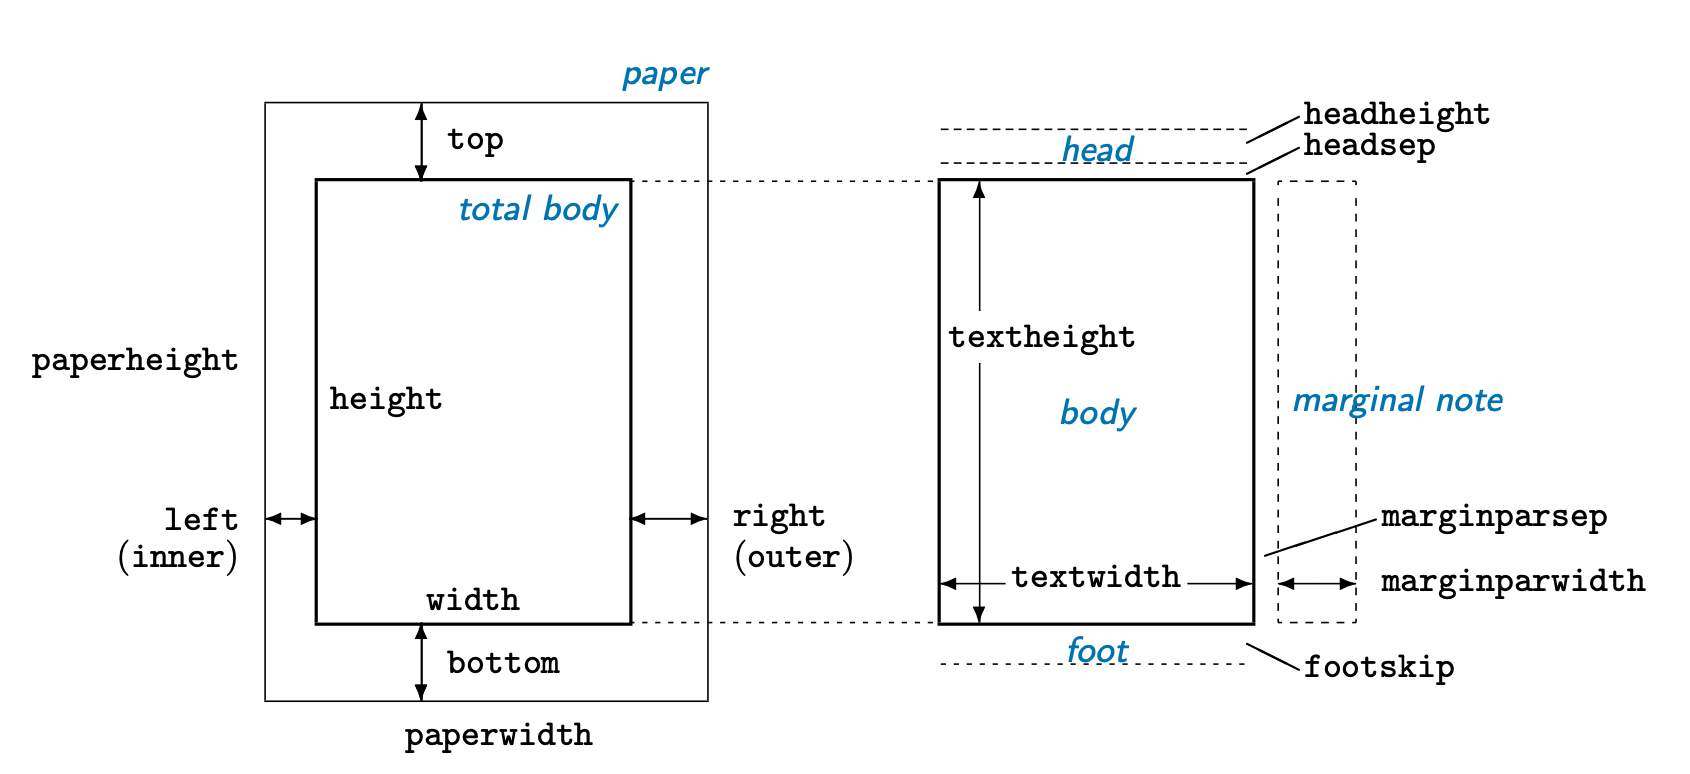
\includegraphics[scale=0.35]{./figures/geometry.png}
            \label{fig: geometry}
    \end{figure}
    \footnotetext{geometry – Flexible and complete interface to document dimensions. \href{https://ctan.org/pkg/geometry}{\textcolor{spruce_dark}{https://ctan.org/pkg/geometry}}.}
\end{frame}

\begin{frame}[fragile]
    \frametitle{Personnalisation de documents - Mise en page}
    Les commandes suivantes pour modifier les dimensions sont équivalentes
    \vfill
    \begin{lstlisting}[xleftmargin=-10mm]
        \usepackage[height=10in, a5paper]{geometry}
    \end{lstlisting}
    \vfill
    \centering
    où
    \vfill
    \begin{lstlisting}[xleftmargin=-10mm]
        \usepackage{geometry}
        \geometry{height=10in, a5paper}
    \end{lstlisting}
\end{frame}

\begin{frame}[fragile]
    \frametitle{Personnalisation de documents - En-têtes, pieds de page et sections}
    Avec \textcolor{vibrant_green}{\textit{fancyhdr}}\footnotemark, on personnalise les en-têtes et pieds de page grâce à l'utilisation d'un nouveau style de page
    \vfill
    \begin{lstlisting}[xleftmargin=1cm]
        \usepackage{fancyhdr}
        \pagestyle{fancy}
    \end{lstlisting}
    \footnotetext{fancyhdr – Extensive control of page headers and footers in \LaTeX. \href{https://ctan.org/pkg/fancyhdr}{\textcolor{spruce_dark}{https://ctan.org/pkg/fancyhdr}}.}
\end{frame}

\begin{frame}[fragile]
    \frametitle{Personnalisation de documents - En-têtes, pieds de page et sections}
    Avec \textcolor{vibrant_green}{\textit{fancyhdr}}\footnotemark, on personnalise les en-têtes et pieds de page grâce à l'utilisation d'un nouveau style de page
    \vfill
    \begin{figure}
        \centering
            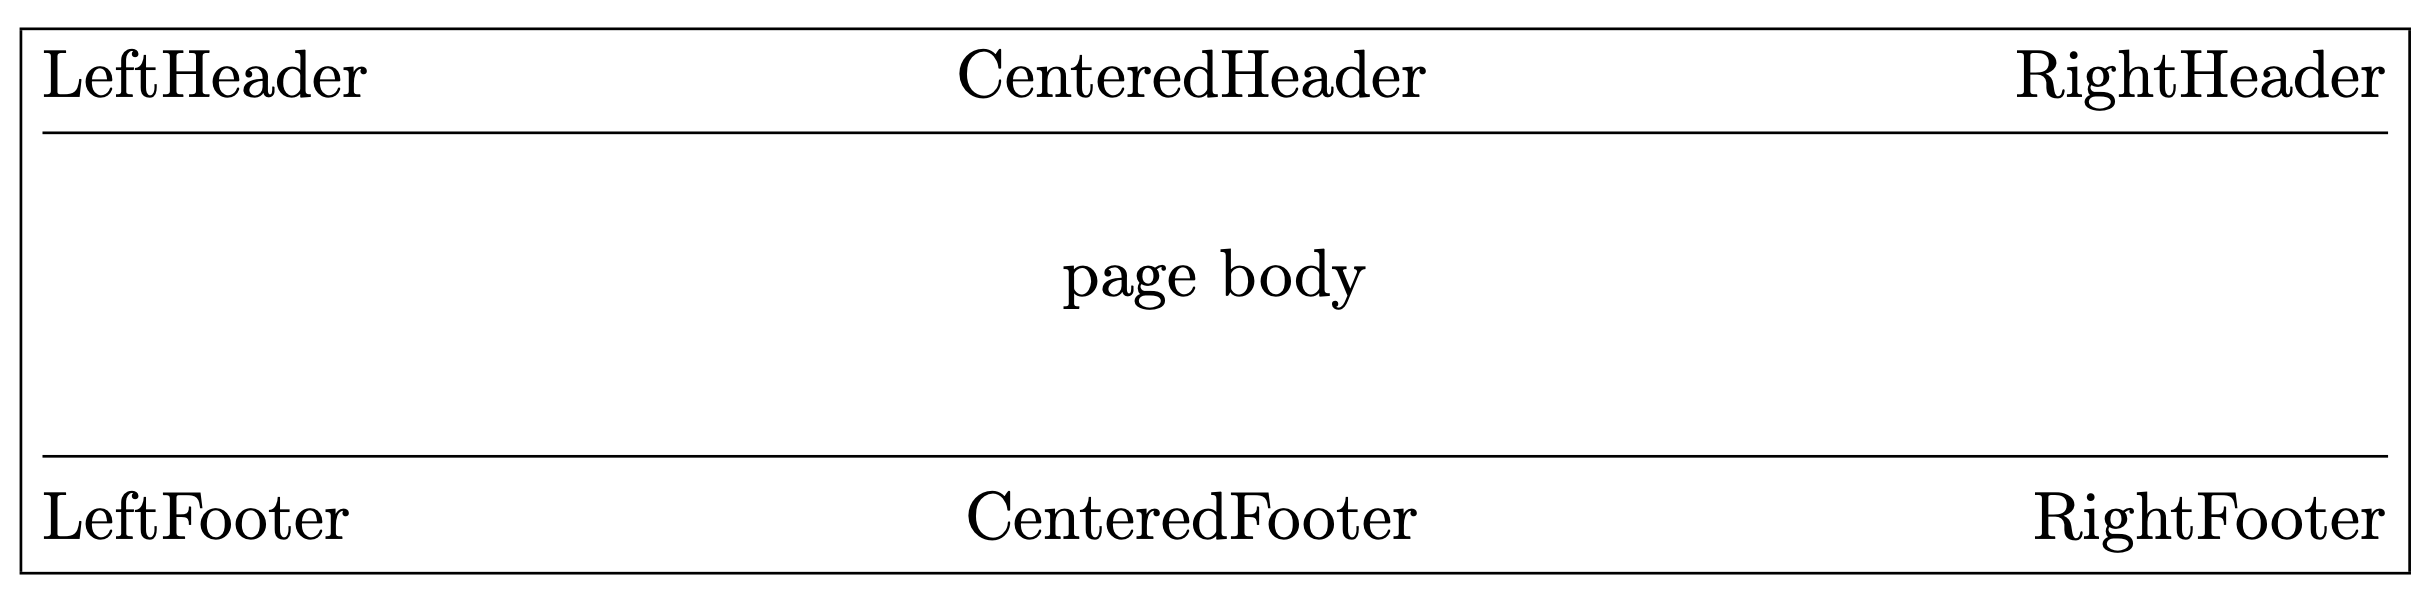
\includegraphics[scale=0.25]{./figures/fancyhdr.png}
            \label{fig: fancyhdr}
    \end{figure}
    \footnotetext{fancyhdr – Extensive control of page headers and footers in \LaTeX. \href{https://ctan.org/pkg/fancyhdr}{\textcolor{spruce_dark}{https://ctan.org/pkg/fancyhdr}}.}
\end{frame}

\begin{frame}[fragile]
    \frametitle{Personnalisation de documents - En-têtes, pieds de page et sections}
    Prenons par exemple le code suivant
    \vfill
    \begin{lstlisting}[xleftmargin=-1.75cm]
        \fancyhead[L,C]{}
        \fancyhead[R]{\textbf{The performance of new graduates}}
        \fancyfoot[L]{From: K. Grant}
        \fancyfoot[C]{To: Dean A. Smith}
        \fancyfoot[R]{\thepage}
        \renewcommand{\headrulewidth}{0.4pt}
        \renewcommand{\footrulewidth}{2pt}
    \end{lstlisting}
    \vfill
\end{frame}

\begin{frame}[fragile]
    \frametitle{Personnalisation de documents - En-têtes, pieds de page et sections}
    Qui permet d'obtenir
    \vfill
    \begin{figure}
        \centering
            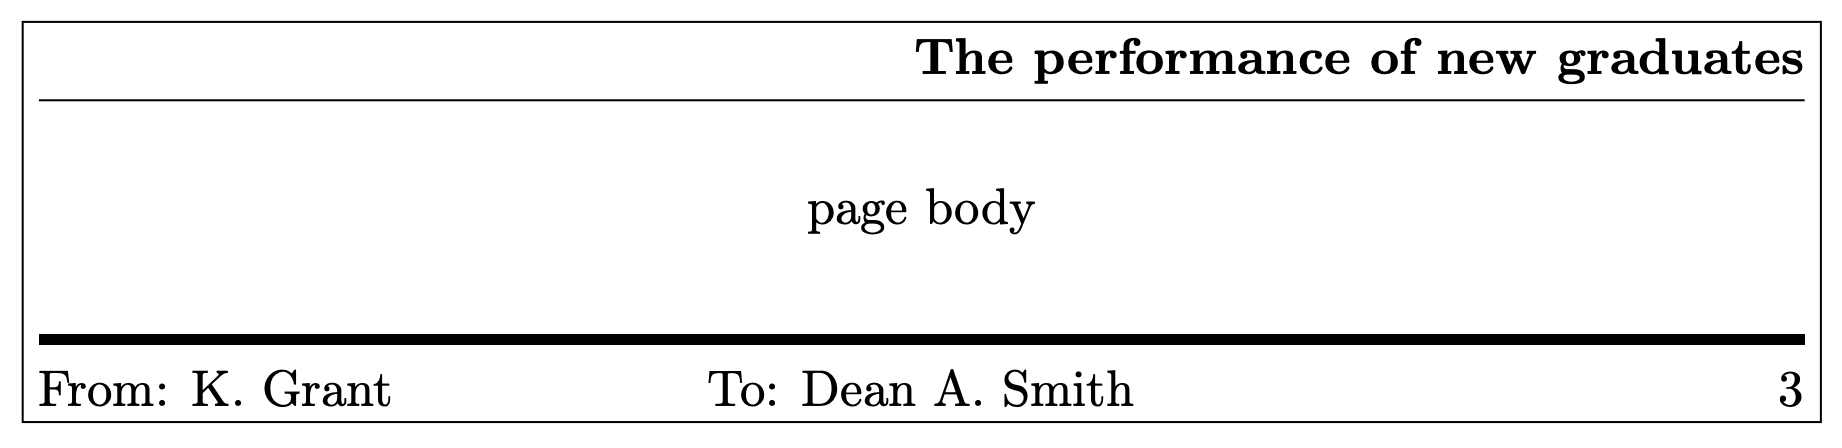
\includegraphics[scale=0.3]{./figures/fancyhdr_2.png}
            \label{fig: fancyhdr_2}
    \end{figure}
    \vfill
\end{frame}

\begin{frame}
    \frametitle{Personnalisation de documents - En-têtes, pieds de page et sections}
    Le module \textcolor{vibrant_green}{\textit{titlesec}}\footnotemark permet de choisir le format des titres de sections, sous-sections et etc.
    \begin{columns}
        \column{0.5\linewidth}
        \begin{figure}
           \centering
            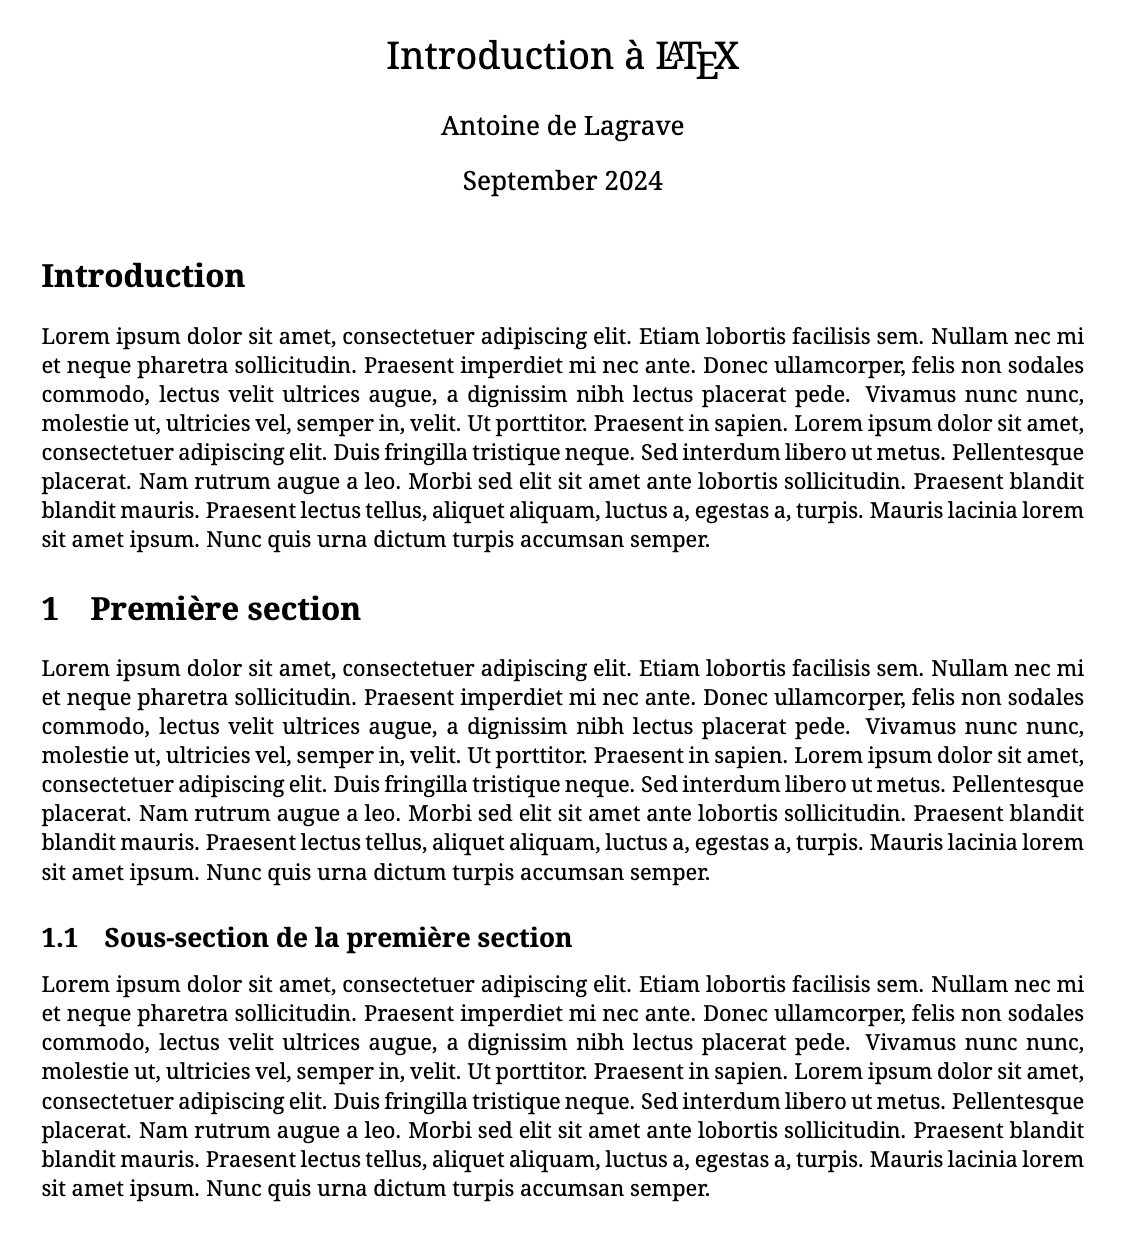
\includegraphics[scale=0.2]{./figures/titlesec.png}
            \label{fig: titlesec}
        \end{figure}
        \column{0.5\linewidth}
        \begin{figure}
           \centering
            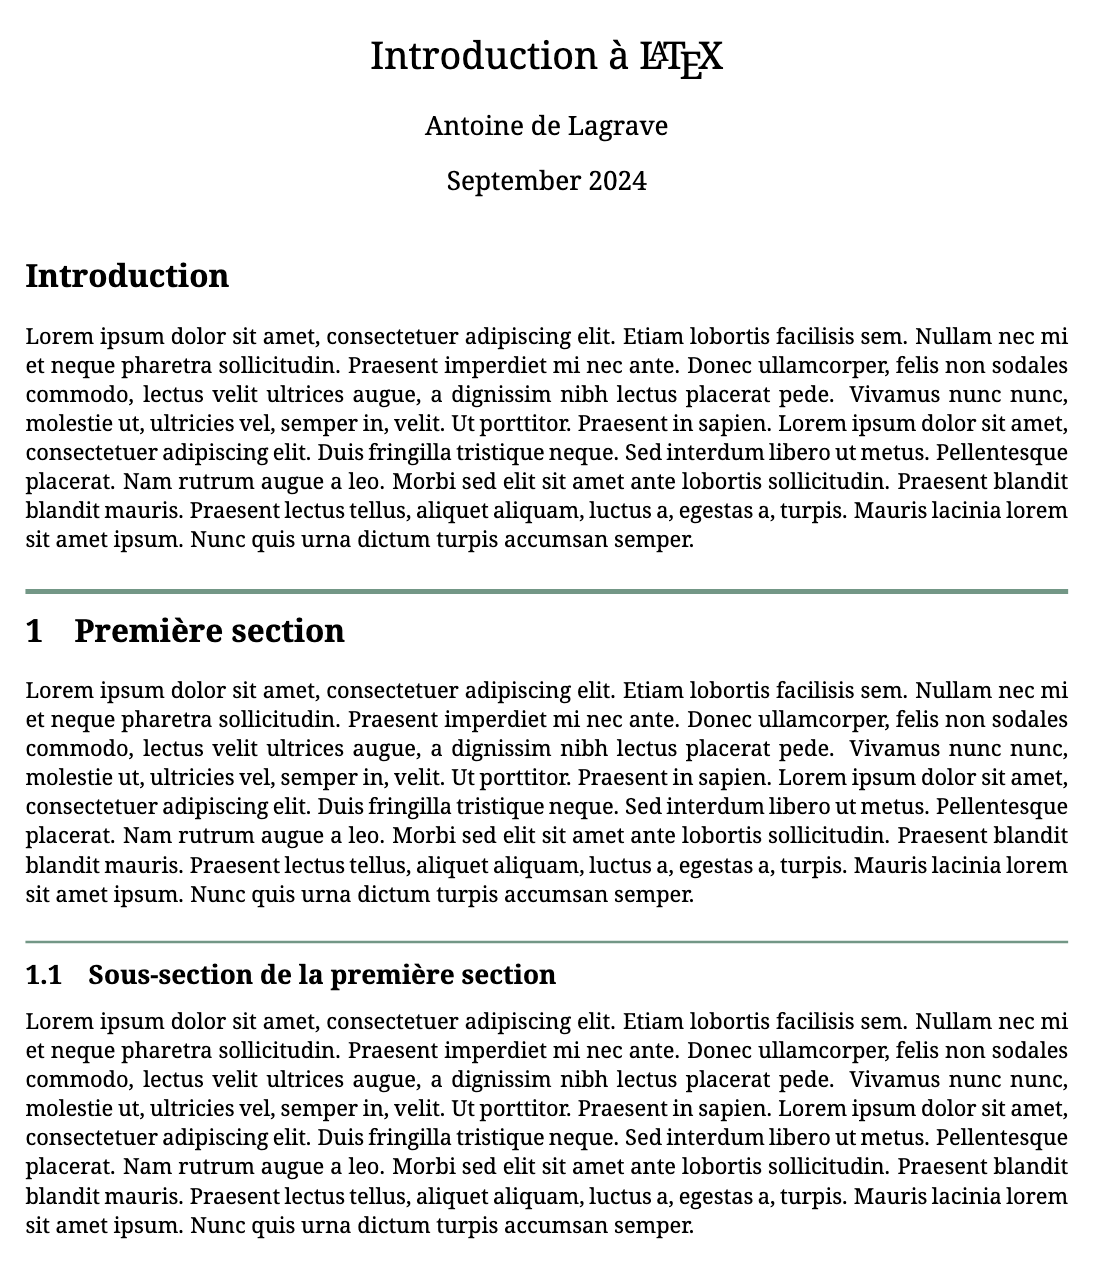
\includegraphics[scale=0.2]{./figures/titlesec_2.png}
            \label{fig: titlesec_2}
        \end{figure}
    \end{columns}
    \footnotetext{titlesec – Select alternative section titles. \href{https://ctan.org/pkg/titlesec}{\textcolor{spruce_dark}{https://ctan.org/pkg/titlesec}}.}
\end{frame}
